\documentclass[aspectratio=169,12pt]{beamer}
\usepackage[utf8]{inputenc}
\usepackage{amsmath, amssymb}
\usepackage{booktabs}
\usepackage{colortbl}
\usepackage{hyperref}
\usepackage{makecell}
\usepackage{ragged2e}
\usepackage{tikz}
\usetikzlibrary{matrix, arrows.meta, positioning, shapes.geometric, calc, tikzmark, shapes.misc, shapes.multipart, fit, decorations.pathreplacing}
\usepackage{tcolorbox}
\usepackage{array}
\usepackage{listings}
\usepackage{pgfkeys}
\usepackage[normalem]{ulem}

\usetheme{Madrid}

% Custom colors
\definecolor{correctgreen}{RGB}{0,150,0}
\definecolor{incorrectred}{RGB}{200,0,0}
\definecolor{counterblue}{RGB}{70,130,255}
\definecolor{highlightyellow}{RGB}{255,230,100}
\definecolor{lightblue}{RGB}{200,230,250}
\definecolor{darkblue}{RGB}{0,100,200}
\definecolor{highlightorange}{RGB}{255,200,100}
\definecolor{memorycolor}{RGB}{200,200,255}
\definecolor{processcolor}{RGB}{255,200,200}
\definecolor{diskcolor}{RGB}{255,255,200}

% PGF keys for configurable macros
\pgfkeys{
  /memblock/.is family,
  /memblock,
  default/.style = {
    width = 3cm,
    height = 0.6cm,
    color = memorycolor,
    text = {},
    label = {}
  },
  width/.estore in = \memblockWidth,
  height/.estore in = \memblockHeight,
  color/.estore in = \memblockColor,
  text/.estore in = \memblockText,
  label/.estore in = \memblockLabel,
}

% Macro for memory blocks
\newcommand{\memoryblock}[2][]{
  \pgfkeys{/memblock, default, #1}
  \node[draw, rectangle, minimum width=\memblockWidth, minimum height=\memblockHeight, 
        fill=\memblockColor, #2] {\memblockText};
  \ifx\memblockLabel\empty\else
    \node[above] at (#2.north) {\small\memblockLabel};
  \fi
}

% Macro for page table entries
\newcommand{\pteentry}[5][]{
  \begin{tikzpicture}[baseline=(current bounding box.center)]
    \node[draw, rectangle split, rectangle split horizontal, 
          rectangle split parts=4, inner sep=2pt, #1] {
      \nodepart{one} V: #2
      \nodepart{two} M: #3
      \nodepart{three} #4
      \nodepart{four} PFN: #5
    };
  \end{tikzpicture}
}

% Macro for address representation
\newcommand{\addressrep}[3][]{
  \begin{tikzpicture}[baseline=(current bounding box.center)]
    \node[draw, rectangle split, rectangle split horizontal, 
          rectangle split parts=2, inner sep=3pt, #1] {
      \nodepart{one} #2
      \nodepart{two} #3
    };
  \end{tikzpicture}
}

% Macro for memory hierarchy diagram
\newcommand{\memoryhierarchy}[1][]{
  \begin{tikzpicture}[
    proc/.style={draw, circle, minimum size=1.5cm, fill=processcolor},
    mem/.style={draw, rectangle, minimum width=2cm, minimum height=3cm, fill=memorycolor},
    disk/.style={draw, cylinder, shape border rotate=90, minimum width=2cm, minimum height=1.5cm, fill=diskcolor},
    #1
  ]
}

\title{Virtual Memory}
\author{Computer Architecture 2340267}
\date{2025, Recitation \#10}

%\subtitle{Computer Architecture}
\begin{document}

\begin{frame}
\titlepage
\end{frame}

\begin{frame}{The Problem}
\begin{columns}
\column{0.6\textwidth}
\begin{itemize}
\item There is a given and limited amount of physical memory
\item How do we divide it among different processes?
\end{itemize}

\column{0.4\textwidth}
\begin{tikzpicture}[scale=0.8]
  \node[draw, circle, fill=processcolor, minimum size=1cm] (cpu) at (0,3) {CPU};
  \node[draw, rectangle, fill=lightblue!50, minimum width=1.5cm, minimum height=0.8cm] (p1) at (-2,1) {Process 1};
  \node[draw, rectangle, fill=lightblue!50, minimum width=1.5cm, minimum height=0.8cm] (p2) at (2,1) {Process 2};
  \node[draw, rectangle, fill=lightblue!50, minimum width=1.5cm, minimum height=0.8cm] (p3) at (0,0) {Process 3};
  \node[draw, rectangle, fill=memorycolor, minimum width=3cm, minimum height=2cm] (mem) at (0,-2.5) {Physical Memory};
  
  \draw[->, thick] (cpu) -- (p1);
  \draw[->, thick] (cpu) -- (p2);
  \draw[->, thick] (cpu) -- (p3);
  \draw[->, dashed] (p1) -- (mem);
  \draw[->, dashed] (p2) -- (mem);
  \draw[->, dashed] (p3) -- (mem);
\end{tikzpicture}
\end{columns}
\end{frame}

\begin{frame}{The Solution: Virtual Memory}
\begin{itemize}
\item Each process uses its own unique \textbf{virtual address space}
\begin{itemize}
  \item Creates the illusion that a single process owns all memory
  \item Process accesses memory only through virtual addresses
\end{itemize}
\item Behind the scenes, the OS maps each process's virtual memory space to physical memory (or disk)
\item When a process accesses a virtual address, hardware translates it to a physical address based on the OS mapping
\end{itemize}
\end{frame}

\begin{frame}{Key Concepts}
\begin{columns}[T]
\column{0.5\textwidth}
\textbf{Physical Memory Terms:}
\begin{itemize}
\item \textbf{Frame}: Physical memory divided into equal units
\item \textbf{PFN} (Physical Frame Number): Frame number in physical space
\end{itemize}

\column{0.5\textwidth}
\textbf{Virtual Memory Terms:}
\begin{itemize}
\item \textbf{Page}: Virtual memory divided into units equal in size to frames
\item \textbf{VPN} (Virtual Page Number): Page number in logical space
\end{itemize}
\end{columns}

\vspace{0.5cm}
\begin{block}{Additional Concepts}
\begin{itemize}
\item \textbf{Swapping}: Using secondary memory to extend memory space
\item \textbf{Demand Paging}: Pages are brought into physical memory only when needed
\end{itemize}
\end{block}
\end{frame}

\begin{frame}{Advantages of Virtual Memory}
\begin{enumerate}
\item \textbf{Memory expansion beyond physical limits} through swapping
\item \textbf{No relocation needed} - each program has its own virtual address space starting at 0
\item \textbf{Easy memory sharing} - multiple PTEs can point to the same physical frame
\begin{itemize}
  \item Special case: Efficient support for process forking
\end{itemize}
\item \textbf{Protection/Isolation} between different process memory spaces
\end{enumerate}
\end{frame}

\begin{frame}{Physical Memory Structure}
\begin{columns}
\column{0.5\textwidth}
Physical memory can be divided into two parts:
\begin{enumerate}
\item \textbf{Upper part}: Contains translation tables for all processes' virtual spaces
\item \textbf{Lower part}: Contains frames holding process memory pages
\end{enumerate}

\vspace{0.3cm}
\textbf{Key principle:}\\
Frame size in physical memory = Page size in virtual memory

\column{0.5\textwidth}
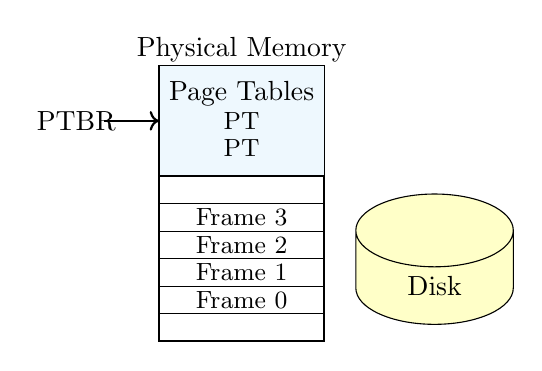
\begin{tikzpicture}[scale=0.7]
  % Physical Memory
  \draw[thick] (0,0) rectangle (3,5);
  \node at (1.5,5.3) {Physical Memory};
  
  % Upper part - Page Tables
  \draw[fill=lightblue!30] (0,3) rectangle (3,5);
  \node at (1.5,4.5) {Page Tables};
  \node at (1.5,4) {\small PT};
  \node at (1.5,3.5) {\small PT};
  
  % Lower part - Frames
  \draw (0,2.5) -- (3,2.5);
  \draw (0,2) -- (3,2);
  \draw (0,1.5) -- (3,1.5);
  \draw (0,1) -- (3,1);
  \draw (0,0.5) -- (3,0.5);
  
  \node at (1.5,2.25) {\small Frame 3};
  \node at (1.5,1.75) {\small Frame 2};
  \node at (1.5,1.25) {\small Frame 1};
  \node at (1.5,0.75) {\small Frame 0};
  
  % PTBR
  \draw[->, thick] (-1,4) -- (0,4);
  \node at (-1.5,4) {PTBR};
  
  % Disk
  \node[draw, cylinder, shape border rotate=90, minimum width=2cm, minimum height=1.5cm, fill=diskcolor] at (5,1) {Disk};
\end{tikzpicture}
\end{columns}
\end{frame}

\begin{frame}{Virtual Address Translation Process}
\begin{columns}
\column{0.6\textwidth}
The CPU addresses only using the process's virtual addresses. To access data in physical memory, we need to translate virtual to physical addresses.

\vspace{0.5cm}
\textbf{Virtual Address Structure:}
\begin{center}
\addressrep{VPN}{Offset}
\end{center}

\begin{itemize}
\item \textbf{VPN}: Virtual Page Number
\item \textbf{Offset}: Displacement from page start to desired byte
\end{itemize}

\column{0.4\textwidth}
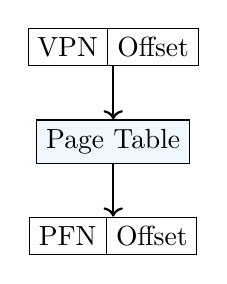
\begin{tikzpicture}[scale=0.8]
  \node[draw, rectangle split, rectangle split horizontal, rectangle split parts=2] (vaddr) at (0,3) {
    \nodepart{one} VPN
    \nodepart{two} Offset
  };
  
  \node[draw, rectangle, fill=lightblue!30] (pt) at (0,1.5) {Page Table};
  
  \node[draw, rectangle split, rectangle split horizontal, rectangle split parts=2] (paddr) at (0,0) {
    \nodepart{one} PFN
    \nodepart{two} Offset
  };
  
  \draw[->, thick] (vaddr) -- (pt);
  \draw[->, thick] (pt) -- (paddr);
\end{tikzpicture}
\end{columns}
\end{frame}

\begin{frame}{Page Table Structure}
\begin{columns}
\column{0.5\textwidth}
\textbf{Page Table Basics:}
\begin{itemize}
\item Each process has its own page table
\item One PTE (Page Table Entry) for each virtual page
\item Index in page table = VPN
\item PTBR (Page Table Base Register) points to current process's page table
\end{itemize}

\column{0.5\textwidth}
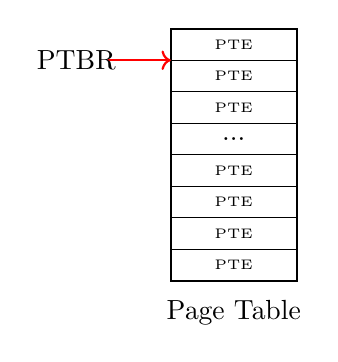
\begin{tikzpicture}[scale=0.8]
  % Page Table
  \draw[thick] (0,0) rectangle (2,4);
  \foreach \y in {0.5,1,1.5,2,2.5,3,3.5} {
    \draw (0,\y) -- (2,\y);
  }
  \node at (1,3.75) {\tiny PTE};
  \node at (1,3.25) {\tiny PTE};
  \node at (1,2.75) {\tiny PTE};
  \node at (1,2.25) {...};
  \node at (1,1.75) {\tiny PTE};
  \node at (1,1.25) {\tiny PTE};
  \node at (1,0.75) {\tiny PTE};
  \node at (1,0.25) {\tiny PTE};
  
  % PTBR arrow
  \draw[->, thick, red] (-1,3.5) -- (0,3.5);
  \node at (-1.5,3.5) {PTBR};
  
  \node at (1,-0.5) {Page Table};
\end{tikzpicture}
\end{columns}

\vspace{0.5cm}
\begin{block}{PTE Address Calculation}
\texttt{PTE\_Address = [PTBR] + VPN * (Size Of One PTE)}
\end{block}
\end{frame}

\begin{frame}{Virtual Memory: Page Table Translation}

%\begin{columns}[T]
%\column{0.4\textwidth}
%\begin{exampleblock}{\scriptsize Address Configuration}
%\scriptsize
%\textbf{PTBR:} 0x1000\\
%\textbf{Virtual Addr:} 30 bits\\
%\textbf{Physical Addr:} 32 bits
%\end{exampleblock}
%
%\column{0.6\textwidth}
%\begin{exampleblock}{\scriptsize Translation Example}
%\scriptsize
%Virtual address mapped through PTE at\\
%\texttt{(00201200 : 940001C0)} base + offset
%\end{exampleblock}
%\end{columns}

%\vspace{0.5cm}

\begin{center}
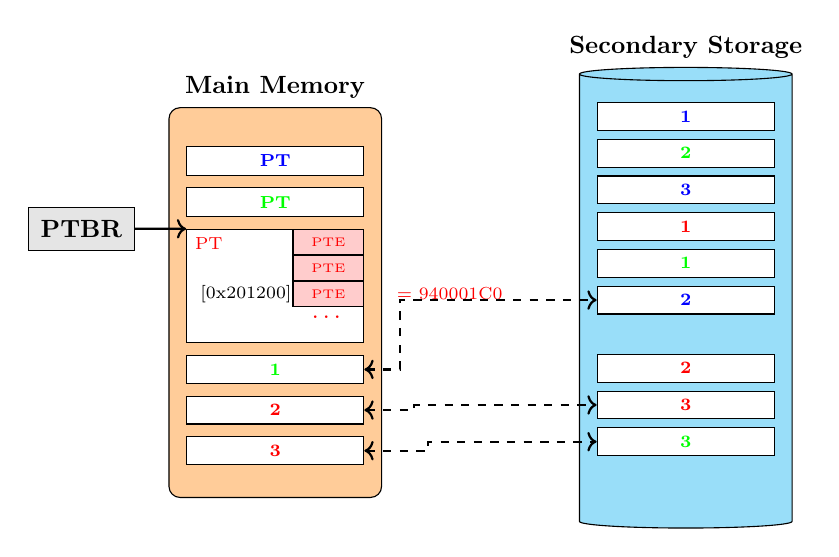
\begin{tikzpicture}[scale=0.9, every node/.style={scale=0.9}]
\tikzset{
  entry/.style={
    draw,
    rectangle,
    fill=white,
    minimum width=2.5cm,
    minimum height=0.35cm,
    font=\bfseries\scriptsize
  },
  pte/.style={
    entry,
    minimum width=1cm,  
    font=\tiny\color{red}
  }
}
% Main Memory (Page Table)
\node[draw, rectangle, fill=orange!40, minimum width=3cm, minimum height=5.5cm, rounded corners] (mainmem) {};
\node[above] at (mainmem.north) {\textbf{Main Memory}};

% Page Table Entries with proper spacing
\node[entry, text=blue] (pt1) at (mainmem.center) [yshift=2cm] {PT};
\node[entry, below=0.15cm of pt1, text=green] (pt2) {PT};
\node[entry, below=0.15cm of pt2, text=red, align=left, minimum height=1.6cm] (pt3) {};
\node[anchor=north west, text=red, align=left, font=\scriptsize] at (pt3.north west) {PT};
\node[pte, fill=red!20, below=0cm of pt3.north east, text=red, anchor=north east] (pte1) {PTE};
\node[pte, fill=red!20, below=0cm of pte1, text=red] (pte2) {PTE};
\node[pte, fill=red!20, below=0cm of pte2, text=red] (pte3) {PTE};
\node[text=red, below=0cm of pte3] (pten) {\ldots};
\node[entry, fill=white, below=0.15cm of pt3.south east, anchor=north east, text=green] (entry1) {1};
\node[entry, fill=white, below=0.15cm of entry1, text=red] (entry2a) {2};
\node[entry, fill=white, below=0.15cm of entry2a, text=blue] (entry2b) {2};
\node[entry, fill=white, below=0.15cm of entry2a, text=red] (entry3) {3};

% PTBR Register
\node[draw, rectangle, fill=gray!20, minimum width=1.5cm, minimum height=0.6cm, left=2cm of pte1.north west] (ptbr) {\textbf{PTBR}};

% Address labels
\node[left, font=\scriptsize, left=-1mm of pte3] at (pte3.west) {[0x201200]};
\node[right, font=\scriptsize, red, right=3mm of pte3] at (pte3.east) {= 940001C0};

% Secondary Storage/Disk
\node[draw, cylinder, shape border rotate=90, fill=cyan!40, minimum width=3cm, minimum height=6.5cm, aspect=0.8, right=2.5cm of mainmem] (storage) {};
\node[above] at (storage.north) {\textbf{Secondary Storage}};

% Storage Pages
\node[entry, text=blue] (page1) at (storage.north) [yshift=-7mm] {1};
\node[entry, below=0.1cm of page1, text=green] (page2a) {2};
\node[entry, below=0.1cm of page2a, text=blue] (page3a) {3};
\node[entry, below=0.1cm of page3a, text=red] (page1b) {1};
\node[entry, below=0.1cm of page1b, text=green] (page1c) {1};
\node[entry, below=0.1cm of page1c, text=blue] (page2b) {2};
\node[entry, below=0.5cm of page2b, text=red] (page2c) {2};
\node[entry, below=0.1cm of page2c, text=red] (page3b) {3};
\node[entry, below=0.1cm of page3b, text=green] (page3c) {3};

% Arrow from PTBR to Page Table
\draw[->, thick] (ptbr.east) -- (pt3.north west);

% Mapping arrows from entries to storage pages
\draw[<->, dashed, thick] (entry1.east) -- ++(0.5,0) |- (page2b.west);
\draw[<->, dashed, thick] (entry2a.east) -- ++(0.7,0) |- (page3b.west);
\draw[<->, dashed, thick] (entry2b.east) -- ++(0.9,0) |- (page3c.west);

\end{tikzpicture}
\end{center}

\vspace{0.3cm}
\begin{exampleblock}{\scriptsize Key Concepts}
\scriptsize
\begin{itemize}
\item PTBR points to page table location in main memory
\item Valid PTEs contain mappings to physical frames in secondary storage
\item Multiple virtual pages can map to the same physical frame
\end{itemize}
\end{exampleblock}

\end{frame}


\begin{frame}{Page Table Entry (PTE) Structure}
\begin{center}
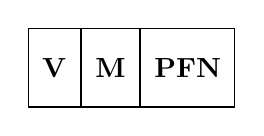
\begin{tikzpicture}
  \node[draw, rectangle split, rectangle split horizontal, rectangle split parts=3, 
        minimum height=1cm, inner sep=5pt] {
    \nodepart{one} \textbf{V}
    \nodepart{two} \textbf{M}
    \nodepart{three} \textbf{PFN}
  };
\end{tikzpicture}
\end{center}

\vspace{0.5cm}
\begin{itemize}
\item \textbf{V (Valid bit)}: Indicates if page is in physical memory
\begin{itemize}
  \item If not, page may be in secondary storage or address is invalid
  \item Invalid access causes \textbf{Page Fault}
\end{itemize}
\item \textbf{M (Modified bit)}: Indicates if page was modified since loading
\begin{itemize}
  \item Used for Write-Back policy
  \item Only write to disk when page is evicted if M=1
\end{itemize}
\item \textbf{PFN}: Physical Frame Number where page resides
\end{itemize}

\vspace{0.3cm}
\textbf{Page Replacement}: LRU (Least Recently Used) policy
\end{frame}

\begin{frame}{Address Translation Diagram}
\begin{center}
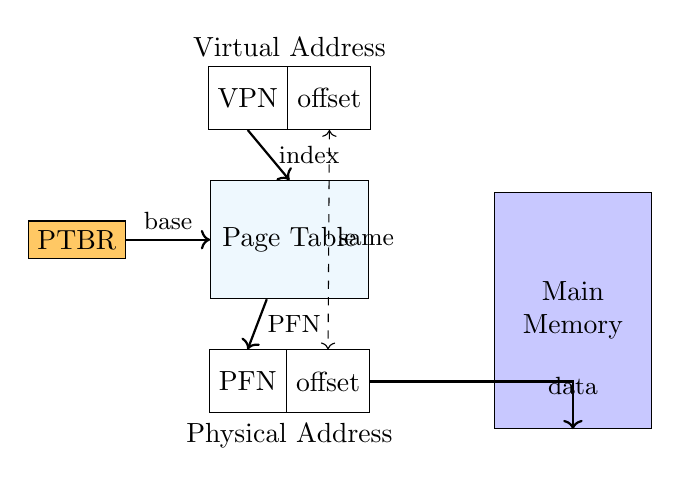
\begin{tikzpicture}[scale=0.9]
  % Virtual Address
  \node[draw, rectangle split, rectangle split horizontal, rectangle split parts=2,
        minimum height=0.8cm] (vaddr) at (0,4) {
    \nodepart{one} VPN
    \nodepart{two} offset
  };
  \node[above] at (vaddr.north) {Virtual Address};
  
  % PTBR
  \node[draw, rectangle, fill=highlightorange] (ptbr) at (-3,2) {PTBR};
  
  % Page Table
  \node[draw, rectangle, fill=lightblue!30, minimum width=2cm, minimum height=1.5cm] (pt) at (0,2) {Page Table};
  
  % Physical Address
  \node[draw, rectangle split, rectangle split horizontal, rectangle split parts=2,
        minimum height=0.8cm] (paddr) at (0,0) {
    \nodepart{one} PFN
    \nodepart{two} offset
  };
  \node[below] at (paddr.south) {Physical Address};
  
  % Memory
  \node[draw, rectangle, fill=memorycolor, minimum width=2cm, minimum height=3cm, align=center] (mem) at (4,1) {Main\\Memory};
  
  % Arrows
  \draw[->, thick] (vaddr.one south) -- (pt.north) node[midway, right] {\small index};
  \draw[->, thick] (ptbr) -- (pt) node[midway, above] {\small base};
  \draw[->, thick] (pt) -- (paddr.one north) node[midway, right] {\small PFN};
  \draw[->, thick] (paddr) -| (mem) node[near end, above] {\small data};
  \draw[<->, dashed] (vaddr.two south) -- (paddr.two north) node[midway, right] {\small same};
\end{tikzpicture}
\end{center}

\textbf{Result}: 2 memory accesses - one for page table, one for data
\end{frame}

\begin{frame}{Example: Virtual Memory System}
\textbf{Given:}
\begin{itemize}
\item Machine without cache
\item Page table in main memory
\item PTBR = 0x1000
\item Content at address 0x00201200 is 0xC0 01 00 94
\item Virtual address: 30 bits
\item Physical address: 32 bits
\item PTE structure (32 bits):
\end{itemize}

\begin{center}
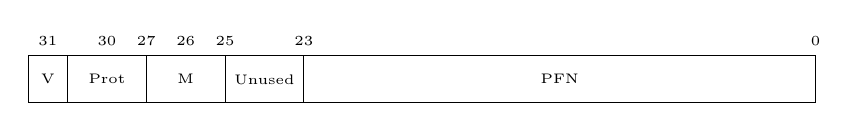
\begin{tikzpicture}
  \draw (0,0) rectangle (10,0.6);
  \draw (0.5,0) -- (0.5,0.6);
  \draw (1.5,0) -- (1.5,0.6);
  \draw (2.5,0) -- (2.5,0.6);
  \draw (3.5,0) -- (3.5,0.6);
  \draw (10,0) -- (10,0.6);
  
  \node at (0.25,0.3) {\tiny V};
  \node at (1,0.3) {\tiny Prot};
  \node at (2,0.3) {\tiny M};
  \node at (3,0.3) {\tiny Unused};
  \node at (6.75,0.3) {\tiny PFN};
  
  \node[above] at (0.25,0.6) {\tiny 31};
  \node[above] at (1,0.6) {\tiny 30};
  \node[above] at (1.5,0.6) {\tiny 27};
  \node[above] at (2,0.6) {\tiny 26};
  \node[above] at (2.5,0.6) {\tiny 25};
  \node[above] at (3.5,0.6) {\tiny 23};
  \node[above] at (10,0.6) {\tiny 0};
\end{tikzpicture}
\end{center}
\end{frame}

\begin{frame}{Example: Address Translation}
\textbf{Question:} A program reads a DW (4 bytes) from virtual address 0x0A100100
\begin{enumerate}
\item What is the physical address?
\item How many memory accesses are needed?
\end{enumerate}

\textbf{Solution:}
\begin{enumerate}
\item Convert to binary: 0x0A100100
\begin{itemize}
  \item = \textcolor{blue}{0000 1010 0001 0000 0000 001}\textcolor{red}{0 0000 0000} (binary)
  \item With 23-bit PFN and 32-bit physical address: \textcolor{red}{offset} = 32 - 23 = 9 bits
  \item \textcolor{blue}{VPN} = upper 21 bits, \textcolor{red}{offset} = lower 9 bits
\end{itemize}
\item Calculate PTE address:
\begin{itemize}
  \item VPN × 4 + PTBR = 0x00201200
\end{itemize}
\item Read PTE content: 0xC0010094
\begin{itemize}
  \item Valid = 1, PFN = 0x0001C0
\end{itemize}
\item Physical address = (PFN $\ll$ 9) + offset = 0x000380A0
\end{enumerate}

\textbf{Answer:} 2 memory accesses (1 for PTE, 1 for data)
\end{frame}

\begin{frame}{TLB - Translation Lookaside Buffer}
\textbf{Problem:} Virtual memory doubles memory access time (need to access page table first)

\textbf{Solution:} TLB - a cache for recently used PTEs

\begin{columns}
\column{0.5\textwidth}
\textbf{How it works:}
\begin{itemize}
\item Check TLB before accessing page table
\item TLB hit → translation in few clock cycles
\item TLB miss → access page table normally
\item Store page table in regular cache too
\end{itemize}

\column{0.5\textwidth}
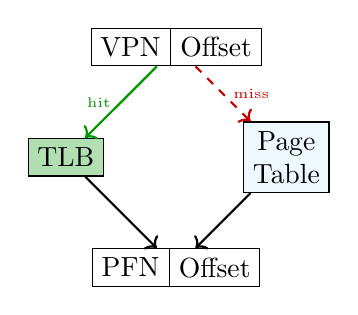
\begin{tikzpicture}[scale=0.7]
  \node[draw, rectangle split, rectangle split horizontal, rectangle split parts=2] (vaddr) at (0,4) {
    \nodepart{one} VPN
    \nodepart{two} Offset
  };
  
  \node[draw, rectangle, fill=correctgreen!30] (tlb) at (-2,2) {TLB};
  \node[draw, rectangle, fill=lightblue!30, align=center] (pt) at (2,2) {Page\\Table};
  
  \node[draw, rectangle split, rectangle split horizontal, rectangle split parts=2] (paddr) at (0,0) {
    \nodepart{one} PFN
    \nodepart{two} Offset
  };
  
  \draw[->, thick, correctgreen] (vaddr) -- (tlb) node[midway, left] {\tiny hit};
  \draw[->, thick, dashed, incorrectred] (vaddr) -- (pt) node[midway, right] {\tiny miss};
  \draw[->, thick] (tlb) -- (paddr);
  \draw[->, thick] (pt) -- (paddr);
\end{tikzpicture}
\end{columns}
\end{frame}

\begin{frame}{Cache and Virtual Memory Optimization}
\textbf{Question:} What speedup can be achieved if $q \geq b + c$?

Where:
\begin{itemize}
\item Virtual memory: $2^n$ bytes, page size: $2^q$ bytes
\item Physical memory: $2^m$ bytes
\item Direct-mapped cache: $2^c$ blocks, block size: $2^b$ bytes
\end{itemize}

\textbf{Answer:} If $q \geq b + c$, then page offset contains both set and displacement fields

\begin{center}
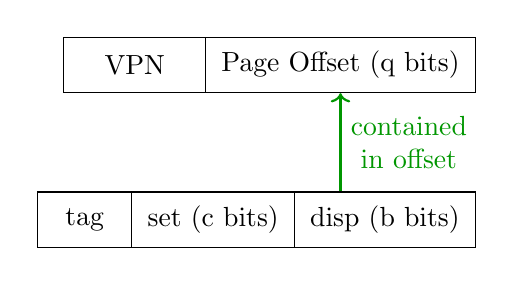
\begin{tikzpicture}[scale=0.9]

% Virtual Address
\matrix[matrix of nodes,
        nodes={draw, minimum height=7mm, inner xsep=2mm, anchor=center},
        column sep=-\pgflinewidth,
        row sep=0pt,
        ampersand replacement=\&] (vaddr) {
  |[minimum width=1.8cm]| VPN \&
  |[minimum width=3.2cm]| Page Offset (q bits) \\
};

% Cache line
\matrix[matrix of nodes,
        nodes={draw, minimum height=7mm, inner xsep=2mm, anchor=center},
        column sep=-\pgflinewidth,
        row sep=0pt,
        below=1cm of vaddr.south east,
        anchor=north east,
        ampersand replacement=\&] (cache) {
  |[minimum width=1.2cm]| tag \&
  |[minimum width=1.8cm]| set (c bits) \&
  |[minimum width=1.2cm]| disp (b bits) \\
};

% Arrow
\draw[<-, thick, correctgreen] 
  (vaddr-1-2.south) 
  -- (cache-1-3.north -| vaddr-1-2.south)
  node[midway, right, align=center] {contained\\in offset};

\end{tikzpicture}
\end{center}

\textbf{Benefit:} Can access cache in parallel with TLB lookup!
\end{frame}

\begin{frame}{Summary}
\begin{itemize}
\item \textbf{Virtual Memory} provides abstraction between logical and physical memory
\item \textbf{Key Benefits:}
\begin{itemize}
  \item Memory larger than physical through swapping
  \item Process isolation and protection
  \item Simplified memory management
  \item Efficient memory sharing
\end{itemize}
\item \textbf{Performance Optimization:}
\begin{itemize}
  \item TLB reduces translation overhead
  \item Clever cache indexing enables parallel access
  \item Page tables can be cached
\end{itemize}
\item \textbf{Trade-offs:}
\begin{itemize}
  \item Extra memory accesses for translation
  \item Page fault handling overhead
  \item Memory needed for page tables
\end{itemize}
\end{itemize}
\end{frame}

\end{document}